\documentclass[12pt,dvipsnames]{article}
\usepackage[utf8]{inputenc}
\usepackage{amsmath}
\usepackage{amssymb}
\usepackage{tikz}
\usetikzlibrary{positioning,arrows.meta}
\usepackage{pgfplots}
\usepackage{pgfplotstable}
\usepackage{tikz}
\usetikzlibrary{positioning,arrows.meta}
\usetikzlibrary{positioning,trees,decorations.pathmorphing,decorations.markings,decorations.pathreplacing,calc,shapes,shapes.geometric,shapes.symbols,patterns,arrows}
\usetikzlibrary{fadings}
\usetikzlibrary{decorations.shapes}
\usepackage{amsmath}
\usepackage{amssymb}
\pgfplotsset{
        compat=1.9,
        compat/bar nodes=1.8,
    }

\begin{document}

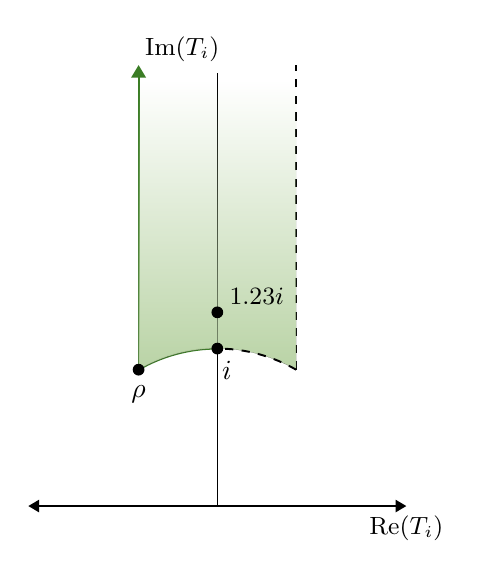
\begin{tikzpicture}[scale=2]
\draw[line width=0.5pt,black,Triangle-] (-1.2,0) -- (0,0);
\draw[line width=0.5pt,black,-Triangle] (0,0) -- (1.2,0) node[below] {\color{black}{\small{Re$(T_i)$}}};
\draw[line width=0.5pt,black] (0,0) -- (0,1);
\draw[line width=0.5pt] (0,1) -- (0,2.75) node[left,xshift=0.15cm,yshift=0.3cm] {\color{black}{\small{Im$(T_i)$}}};
\draw[dashed,line width=0.7pt] (0.5,0.866) -- (0.5,2.8);
\draw[line width=0.7pt,OliveGreen,-Triangle] (-0.5,0.866) -- (-0.5,2.8);
\draw[line width=0.7pt,OliveGreen] (-0.5,0.866) arc[start angle=120, end angle=90,radius=1cm];
\draw[fill=OliveGreen!30,path fading=north,line width=0.01pt](0,1)--(0,2.7)--(-0.5,2.7)--(-0.5,0.866) arc[start angle=120, end angle=90,radius=1cm,line width=0.001pt];
\draw[fill=OliveGreen!30,path fading=north,line width=0.001pt](0,1)--(0,2.7)--(0.5,2.7)--(0.5,0.866) arc[start angle=60, end angle=90,radius=1cm,line width=0.001pt];
\draw[dashed,line width=0.7pt] (0.5,0.866) arc[start angle=60, end angle=90,radius=1cm];
\node at (0,1)[circle,fill=Black,inner sep=1.5pt,label={[xshift=0.12cm,yshift=-0.6cm]:$i$}]{};
\node at (-0.5,0.866)[circle,fill=Black,inner sep=1.5pt,label={[xshift=0cm,yshift=-0.63cm]:$\rho$}]{};
\node at (0,1.23)[circle,fill=Black,inner sep=1.5pt,label={[xshift=0.5cm,yshift=-0.1cm]:\small{$1.23i$}}]{};
% (0.5,1.65) -- (1.2,2.3);
\end{tikzpicture}

\end{document}